\subsection{Le recyclage, une obligation}

Le recyclage est défini par le Larousse  comme étant l'\og{}\textit{ensemble des techniques ayant pour objectif de récupérer des déchets et de les réintroduire dans le cycle de production dont ils sont issus}\fg{}. L'un des objectifs de l'Europe est de réduire les déchets. Une série de lois ont donc été adoptées par l'union européenne, puis retranscrite par la France. 

La directive européenne 2012/19/UE du 4 juillet 2012, retranscrite dans le droit français par le décret 2014-928 du 19 août 2014 oblige  les magasins dont la surface est supérieure à $400m^2$ à accepter n'importe quel \textit{DEEE} de petite taille, et ce sans obligation d'achat pour le consommateur. 

Depuis 2005, un décret (articles R. 543-172 à R. 543-206 du code de l'environnement) mis en place pour transposer% terme officiel
 une directive européenne, oblige le consommateur à recycler un objet électronique lorsqu'il en achète un nouveau. Pour ce faire, il peut le ramener dans le lieu d'achat du nouveau produit, ou bien en déchetterie, ou encore dans les réseaux solidaire comme Emmaüs.

\begin{wrapfigure}{l}{0.3\linewidth}
~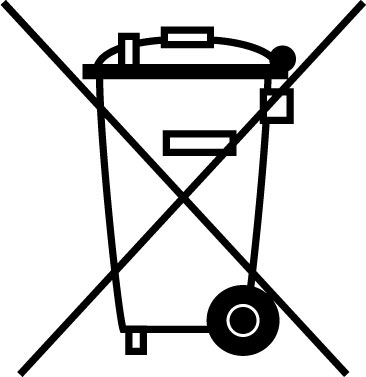
\includegraphics[scale=0.33]{Rsc/pictopoubellebarree.jpg} 
\caption{Pictogramme instauré par la loi de 2006}
\label{fig::picPoubelleBarree}
\end{wrapfigure} 
La loi a également mis en place le pictogramme représentant une poubelle barrée (figure \ref{fig::picPoubelleBarree}), présent sur chaque objet électronique, pour rappeler au consommateur qu'il lui est nécessaire de recycler le nouveau produit à la fin de son utilisation.

Plus flagrant peut être, la loi a instauré la taxe d'éco-participation. Celle ci rend le consommateur contribuable au recyclage. Elle est calculée à partir du coup de collecte du produit (donc de son poids et de sa taille) et du coup de traitement lors du recyclage. Ainsi, les prix varient d'un centime d'euro pour un GPS à 13\euro pour un congélateur. 

La taxe est directement payé par le consommateur. Elle est collectée par le distributeur (\textit{but}, \textit{carrefour}, \dots). Une partie est donnée aux constructeurs (ceux qui acceptent les \textit{DEEE}),le reste est distribuée aux différents éco-organisme. 

Les éco-organismes sont divisés en trois entités différentes : les organismes de collecte, les organismes de traitement et les organismes de remise en état. Ces trois institutions différentes vont toucher une division correspondant au service fourni lors du recyclage. 

\medbreak


\textit{Envie 44}  est une réseau solidaire basé à Nantes (dont le directeur adjoint a été interviewé par \textit{Télénantes} affirme toucher 20\% de ses recettes grâce aux subventions de l'état\cite{7andco}.

L'association récupère les \textit{DEEE} auprès des producteurs de déchets électroniques (principalement des administration : mairie, hôpital) et se charge du recyclage. 

Pour \textit{Envie 44}, le recyclage se divise en deux parties. 
\begin{itemize}
\item 12\% des DEEE étaient rénovés en 2008. Il estimait alors que ce taux pourrait monter jusqu'à 25\%, mais pas plus : 3 machines sont nécessaire pour en réparer une. En 2014, l'entreprise a vendu plus de 7000 articles issus du recyclage. 
\item le reste est envoyé dans des centres de traitement, à Rennes et à Angers.
\end{itemize}

Pour l'entreprise, l'éco-participation a été un véritable moteur, qui lui a permis de se développer. Elle compte aujourd'hui 92 employés. Le filon a attiré de nombreuses nouvelles entreprises de recyclage, fondées à la suite du décret. 


\bigbreak

Ainsi certaines associations ou entreprises profitent des \textit{DEEE} pour créer de nouveaux produits fonctionnels. Cependant, moins d'un quart des déchets que récupère \textit{Envie 44} est rénové. Nous disions plus tôt que le reste des déchets étaient envoyés vers  des centres de traitements. 

D'après \textit{ADEME}\cite{ADEME_unite_traitement}, \og \textit{le terme " traitement " correspond à la transformation des fractions valorisables des déchets}  \fg{}. Concrètement, si une partie des déchets est triée et revalorisée, nos \textit{DEEE} sont principalement incinérés, avec ou sans valorisation énergétique. 

Autre point surprenant : les déchets de Nantes sont envoyés à Angers ou à Rennes (90 ou 110 km).   Les déchets sont donc déplacés, puis brulés. La production de \textit{CO2} n'est donc pas négligeable. 

\bigbreak

Ainsi, le recyclage des \textit{DEEE} est obligatoire. Une partie des déchets est réinjecté dans le marché suite à une rénovation, cependant, une partie des objet n'ayant pas pu être sauvé sera brûlé. Le recyclage reste malgré tout une bonne solution, cependant des progrès restent à faire. 
\medbreak
Une autre solution pour émettre moins de déchets serait de penser le produit à la base pour qu'une pièce défectueuse n'engendre pas la mort totale du produit. 
